%!TEX root = ../Thesis.tex

\chapter[Rekonstruktion von Fahrzeugtrajektorien aus Luftaufnahmen]
        {Rekonstruktion von Fahrzeug-\\\hspace{1em}trajektorien aus Luftaufnahmen}
\label{sec:position_extraction}

In diesem Kapitel wird erläutert, wie aus Luftaufnahmen Trajektorien von Fahrzeugen rekonstruiert werden können.

\begin{theorem}[Trajektorie]
    Eine Trajektorie beschreibt die Bewegungsbahn eines Objektes durch den Raum.
    In der Regel wird sie als Sequenz von Punkten in einem n-dimensionalen Koordinatensystem dargestellt.
    Alternative Darstellungen unter Verwendung von Richtungsvektoren oder des zusätzlichen
    Einbezugs von Geschwindigkeitsinformationen et cetera sind ebenso möglich.
\end{theorem}

Trajektorien sind grundsätzlich die wichtigste Informationsquelle bei der Analyse des Fahrverhaltens aus Luftbeobachtungen.
Eine Rekonstruktion von Fahrzeugtrajektorien wird im Rahmen dieser Arbeit nicht umgesetzt,
allerdings ist es wichtig ein Grundverständnis der hierzu benötigten Methoden und Schritte zu besitzen,
um die Trajektoriedaten und die darin enthaltenen Defekte interpretieren zu können.

Nachfolgend wird beschrieben, wie Fahrzeuge in Videoaufnahmen erkannt und verfolgt
werden können, um anschließend deren Positionen in einem Weltkoordinatensystem zu bestimmen. Am Ende des Kapitels
werden einige Herausforderungen, welche bei der Rekonstruktion der Trajektorien auftreten, aufgezeigt.

\section{Erkennung und Verfolgung von Fahrzeugen in Videoaufnahmen}

Es existieren unterschiedliche Ansätze, welche zur Erkennung und Verfolgung von Fahrzeugen in Videoaufnahmen
eingesetzt werden können.

Ein Verfahren, welches gute Ergebnisse liefern kann, aber mit einem nicht unerheblichen manuellen Aufwand verbunden ist,
ist das \textit{Supervised-Tracking}. Hierbei werden initial manuell ausgewählte Bildbereiche, sogenannte
\textit{Region of Interests} (\acrshort*{roi}s), automatisch mithilfe eines erlernten Klassifikators verfolgt.
Dieser Klassifikator muss zwischen Fahrzeugen und ihrer Umgebung unterscheiden können \cite[]{Grabner}.
Der Supervised-Tracking Ansatz entspricht, aufgrund der notwendigen manuellen Detektion von Fahrzeugen, nichtmehr
dem aktuellen Stand der Technik.

Modernere Verfahren detektieren Fahrzeuge in Videoaufnahmen vollautomatisch und nutzen einen separaten
Tracking-Schritt, um anhand der Einzeldetektionen Trajektorien zu erstellen. Ein solcher zweistufiger
Ansatz wird auch in der Anwendung \textit{Vehicle-Tracker} eingesetzt. Er wird nachfolgend in groben
Zügen beschrieben.

\subsection{Fahrzeug-Detektion}

In der Detektionsphase werden die Positionen der Fahrzeuge in der Videoaufnahme ermittelt.
Üblicherweise wird die Detektion für jedes Frame des Videos ausgeführt.
Erkannt werden die Fahrzeuge in der Anwendung \textit{Vehicle-Tracker} mithilfe von Tensorflow\footnote{Tensorflow - \url{https://www.tensorflow.org/}}.
Das quelloffene Machine-Learning Framework bietet in seiner \textit{Object DetectionAPI}
verschiedene Netzwerk-Architekturen und vortrainierte Modelle an, welche zur Erkennung und Klassifizierung
von Objekten eingesetzt werden können \cite[]{Huang2018}. Die angebotenen neuronalen Netze sind Weiterentwicklungen
von \textit{Convolutional Neural Networks} (\acrshort*{cnn}s), welche sich gut zur maschinellen Verarbeitung
von Bilddaten eignen.

In Abbildung \ref{fig:grund_structure_cnn} ist der Aufbau eines CNN dargestellt.
Ein genaues Verständnis der Funktionsweise eines solchen Netzwerks ist im Fall dieser Arbeit nicht notwendig.
Grundlegend besteht es allerdings aus zwei Komponenten: Der erste Teil ist für
die \textit{Merkmals-Extraktion} verantwortlich, während der zweite Teil der \textit{Klassifizierung} dient.
In der ersten Phase extrahiert das Netzwerk aus einem Bild Merkmale, mittels
welcher die zu erkennenden Objekte beschrieben werden können. Nach welchen Kriterien in einem Bild gesucht wird,
wird während der Trainingsphase des Netzes ermittelt.
Anhand der Merkmale werden die Positionen der gesuchten Objekte im Bild bestimmt.
Um welches Objekt es sich an einer bestimmten Position handelt, wird anschließend vom sogenannten
\textit{Fully-Connected-Layer} ermittelt. \cite[]{Cornelisse2018}

\begin{figure}[H]
    \centering
    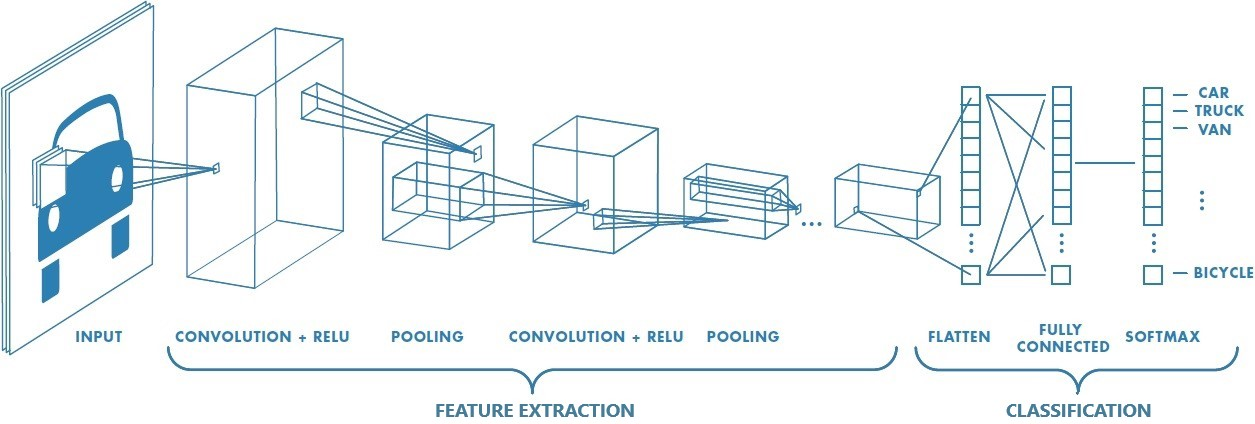
\includegraphics[width=0.95\linewidth]{resources/img/grundlagen/TrajectoryReconstruction/cnn_structure}
    \caption[Aufbau eines CNN]{Aufbau eines CNN \cite[]{PatelShyamal2017}}
    \label{fig:grund_structure_cnn}
\end{figure}

Im Fall der Tensorflow Object Detection API werden die Positionen der erkannten Objekte über sogenannte
\textit{Bounding-Boxes} definiert. Die Lage und Größe dieser rechteckigen Markierungen im Bild, wird über
zwei Pixel-Koordinaten angegeben. \cite[]{Huang2018}

\subsection{Fahrzeugverfolgung}

Nachdem in jedem Video-Frame einer Aufnahme die Positionen der Fahrzeuge ermittelt wurden,
müssen aus diesen Einzeldetektionen anschließend Trajektorien erstellt werden.
Hierzu müssen alle Positionsinformationen, welche von einem Fahrzeug stammen, einer Bewegungsbahn zugeordnet werden.
Eine solche Zuordnung ist nicht trivial, da nie bekannt ist, an welcher Position sich ein Fahrzeug im
nächsten Video-Frame befinden wird.

Ein Algorithmus zur Rekonstruktion der Trajektorien aus den Einzeldetektionen muss die Fahrzeuge im Video
verfolgen. Um dies zu erreichen, kann beispielsweise, wie in der Anwendung \textit{Vehicle-Tracker},
ein auf einem Partikel-Filter basierender Tracking-Ansatz verwendet werden.
Ein Partikel-Filter, auch bekannt als \textit{sequenzielle Monte-Carlo-Methode}, dient der Schätzung
des Zustandes eines dynamischen Systems basierend auf vorherigen Messwerten.
Bei der Fahrzeugverfolgung kann mithilfe eines Partikel-Filters ermittelt werden, an welcher Stelle sich
ein solches im Video-Frame $t$, basierend auf dessen vorherigen Positionen, vorraussichtlich befindet \cite[]{Apeltauer2015}.
Um eine Vorhersage für Frame $t$ einer Detektion aus Frame $t$ zuzuweisen, und so Trajektorien aus diesen zu erstellen,
kann der \textit{Ungarische Algorithmus} von Harold W. Kuhn eingesetzt werden, welcher eine optimale
Zuweisung berechnet \cite[]{Szottka2011}. Kann eine Vorhersage keiner Detektion zugeordnet werden,
so wird eine neue Trajektorie initialisiert.

Mithilfe dieses Verfahrens lassen sich Fahrzeugtrajektorien Frame-für-Frame anhand vorher ermittelter
Detektionen rekonstruieren. Messlücken in den Detektionen können unter Verwendung eines Partikel-Trackers
außerdem interpoliert werden, solange diese nicht zu groß sind.
Die erstellten Trajektorien beschreiben die Bewegungen der Fahrzeuge anschließend in Pixel-Koordinaten.

\section{Positionsbestimmung in Videoaufnahmen}
\label{sec:grund_mapMatching}

Nachdem die Positionen der Fahrzeuge in Pixel-Koordinaten bestimmt wurden, müssen diese in 3D Weltkoordinaten
umgewandelt werden, um die genauen Fahrzeugpositionen auf der Straße zu erhalten. Dank der Verwendung eines
stationären Weltkoordinatensystems mit Einheit Meter, lassen sich zudem reale Entfernungen
in der Aufnahme ermitteln, was beispielsweise für die Bestimmung der Fahrzeuggeschwindigkeiten sehr wichtig ist.

Um eine Bildkoordinate in eine Weltkoordinate überführen zu können, müssen vorher verschiedene Kameraeigenschaften
ermittelt werden. Hierzu ist es wichtig ein grundlegendes Verständnis von der Funktionsweise einer Kamera zu besitzen.
Anhand eines Lochkameramodells lässt sich die Funktionsweise der Bildprojektion erklären.
Ein solches Modell ist in Abbildung \ref{fig:grund_pinhole_model} dargestellt.

\begin{figure}[H]
    \centering
    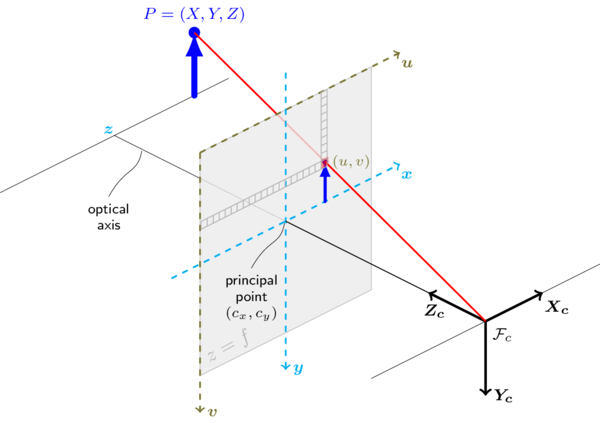
\includegraphics[width=0.55\linewidth]{resources/img/grundlagen/TrajectoryReconstruction/pinhole_camera_model}
    \caption[Bildprojektion im Lochkameramodell]
            {Projektion eines Punktes P auf die Projektionsfläche einer Lochkamera \cite[]{DevTeamOpenCV2018}}
    \label{fig:grund_pinhole_model}
\end{figure}

In einer Lochkamera fällt Licht durch eine kleine Öffnung auf eine Projektionsfläche. Es werden keine Linsen
zur Bündelung des Lichtes eingesetzt. Für die Projektion eines Punktes $P$ auf diese Fläche müssen vier
Bezugssysteme berücksichtigt werden \cite[]{Jahne2012}:

\begin{enumerate}
    \item Das \textbf{Weltkoordinatensystem} ist ein stationäres Bezugssystem, dessen Ursprung sich an einem beliebigen Punkt
            im aufgenommenen Raum befindet. Über dieses System werden Weltkoordinaten $P = (X, Y, Z)$ definiert.
    \item Das \textbf{Kamerakoordinatensystem} hat seinen Ursprung im Punkt $F_c$, der Öffnung des Kamerasystems.
            Es definiert Punkte $P = (x_c,\ y_c,\ z_c)$ relativ zur Kamera.
    \item Das \textbf{Projektionskoordinatensystem} hat seinen Ursprung im Punkt $C = (c_x,\ c_y)$ der Projektionsfläche.
            Über es werden zweidimensionale Punkte $P' = (x_p, y_p)$ definiert.
    \item Der Ursprung des \textbf{Bildschirmkoordinatensystems} ist die linke obere Ecke der Projektionsfläche.
            Über es werden Punkte $P' = (u,\ v)$ in der Einheit Pixel definiert.
\end{enumerate}

Unter Berücksichtigung dieser Bezugssysteme können die sogenannten \textit{intrinsischen} und
\textit{extrinsischen} Kameraparameter bestimmt werden.

\subsubsection{Intrinsische Kamera- und Verzeichnungsparameter}

Die intrinsischen Kamera- und Verzeichnungsparameter sind abhängig von der Bauart der Kamera und gelten
daher für alle Aufnahmen, welche mit der selben Hardwarekonfiguration getätigt werden.
Die Parameter $c_x$ und $c_y$, welche die Bildmitte festlegen, und die
horizontale und vertikale Brennweite $f_x$ und $f_y$ definieren die intrinsischen Kameraparameter.
Mit ihrer Hilfe lässt sich eine Kameramatrix der Form

\begin{ceqn}
\begin{align}
A =
 \begin{bmatrix}
  f_x & 0 & c_x \\
  0 & f_y & c_y \\
  0 & 0 & 1
 \end{bmatrix}
\end{align}
\end{ceqn}

bilden.
Die Verzeichnungsparameter sind abhängig von den Linsen, welche in einer Kamera verwendet werden. Diese sorgen
für eine radiale und tangentiale Verzeichnung des Bildes. Die Parameter $k_1$, $k_2$ und $k_3$ definieren die
radiale und $p_1$ und $p_2$ die tangentiale Verzeichnung. \cite[]{Meissner2007}

Die intrinsischen Kamera- und Verzeichnungsparameter können durch ein Kalibrierungsverfahren bestimmt werden.
Computervision Bibliotheken wie OpenCV bieten hierfür Hilfsfunktionen an \cite[]{DevTeamOpenCV2018}.

\subsubsection{Extrinsische Kameraparameter}

Die extrinsischen Kameraparameter definieren, wie ein Punkt $P_w$ des 3D-Weltkoordinaten-systems in einen 3D-Punkt $P_c$
des Kamerakoordinatensystems überführt wird. Die Transformation ist in Gleichung \ref{eq_point_transformation}
beschrieben:

\begin{ceqn}
\begin{align}
\label{eq_point_transformation}
    P_c = R P_w + t
\end{align}
\end{ceqn}

$R$ und $t$ sind die extrinsischen Kameraparameter. $R$ ist die sogenannte Rotationsmatrix, welche
die Drehung der Kamera um die X, Y und Z-Achse beschreibt. $t$ ist der Translationsvektor,
welcher angibt, wo sich der Ursprung des Weltkoordinatensystems relativ zur Öffnung der Kamera befindet. \cite[]{Jahne2012}

Die extrinsischen Parameter einer Aufnahme lassen sich mithilfe der intrinsischen Kamera- und Verzeichnungsparameter
und mindestens sechs Weltkoordinaten, welche Bildschirmkoordinaten zugeordnet werden können, bestimmen. Bibliotheken
wie OpenCV bieten auch hierfür Funktionen an. Mithilfe der Weltkoordinaten lässt sich zudem auch das Weltkoordinatensystem
definieren.

\subsubsection{Transformation von Bildschirmpositionen in Weltkoordinaten}

Die Transformation einer Weltkoordinate in eine Bildschirmposition ist, ohne Berücksichtigung der Verzeichnung,
gegeben durch die Formel \ref{eq_point_transformation2} \cite[]{DevTeamOpenCV2018}. $s$ ist hier ein konstanter
Skalierungsfaktor.

\begin{ceqn}
\begin{align}
\label{eq_point_transformation2}
    s\ \big[u\ v\ 1\big]^T = A \big[R\ t\big]\ P_w
\end{align}
\end{ceqn}

Da bei der Projektion vom Weltkoordinatensystem ins Bildschirmkoordinatensystem eine Dimensionsinformation
verloren geht, muss bei der Rücktransformation diese extra bestimmt oder geschätzt werden. Liegt ein Punkt
auf der Ebene, welche von der X- und Y-Achse des Weltkoordinatensystems beschrieben wird, kann für dessen
Höhe $z = 0$ verwendet werden.
Die Position eines Weltpunktes $P$ kann so mithilfe des folgenden Gleichungssystems bestimmt werden:

\begin{ceqn}
\begin{align}
\label{eq_point_transformation3}
    P = \big[X\ Y\ 0\big]^T = R^{-1}\Big(sA^{-1} \big[u\ v\ 1\big]^T - t\Big)
\end{align}
\end{ceqn}

In der Anwendung \textit{Vehicle-Tracker} werden auf diese Weise alle Bildschirmkoordinaten der Trajektorien
in Weltkoordinaten umgewandelt. Dieser Vorgang wird \textit{MapMatching} genannt.

\section{Herausforderungen bei der Rekonstruktion von Fahrzeugtrajektorien}
\label{sec:grund_challenges_reconstruction}

Unabhängig vom eingesetzten Verfahren zur Erkennung und Verfolgung von Fahrzeugen in Videoaufnahmen
existieren diverse Herausforderungen bei der Rekonstruktion von Trajektorien. Nachfolgend sind
häufig auftretende Probleme und deren Auswirkungen beschrieben.

\subsubsection*{False-Positive und False-Negative Detektionen}
Mit \textit{False-Positive Detektionen} sind Objekterkennungen gemeint, welche kein Fahrzeug zeigen.
Dieses Problem tritt häufig dann auf, wenn das für die Detektion eingesetzte neuronale Netz nicht ausreichend trainiert wurde.
Fälschlicherweise detektierte Objekte können beispielsweise Fußgänger, Fahrradfahrer oder auch Gebäude- und Lanschaftsabschnitte sein.
In Abbildung \ref{fig:grund_false_positive_detections} sind False-Positive Detektionen von Fußgängern
und einem Schild auf einem Grünstreifen zu sehen.
Aufgrund von False-Positive Detektionen befinden sich in Trajektoriedatensätzen Bewegungsbahnen, welche nicht zu
Fahrzeugen gehören, häufig außerhalb der Fahrbahnen verlaufen und meist sehr kurz sind.

\begin{figure}[H]
    \centering
    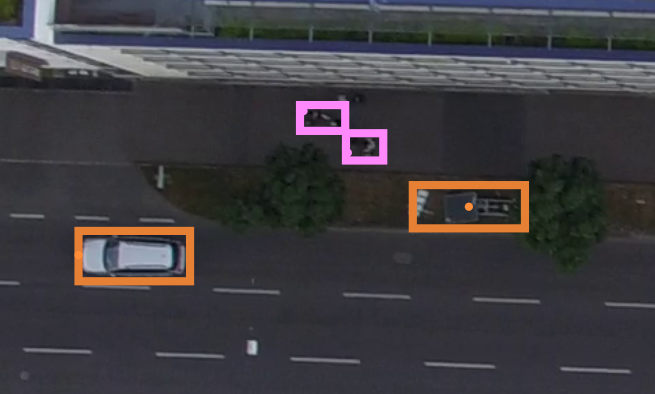
\includegraphics[width=0.45\linewidth]{resources/img/grundlagen/TrajectoryReconstruction/challenges/False-Positives}
    \caption[False-Positive Detektionen]{False-Positive Detektionen von Fahrzeugen in einer Luftaufnahme}
    \label{fig:grund_false_positive_detections}
\end{figure}

Wird ein Fahrzeug in einer Aufnahme nicht erkannt und verfolgt, so handelt es sich dabei um eine
\textit{False-Negative Detektion}.
Die häufigsten Ursachen für diese Problematik sind schlechte Belichtungsverhältnisse oder eine zu geringe
Größe der Fahrzeuge in der Videoaufnahme.
In den Trajektoriedaten äußern sich False-Negative Detektionen primär durch das Fehlen von Bewegungsbahnen
oder deren zu frühen Abbruch.

\subsubsection*{Verdeckungen der Fahrbahn}

In Luftaufnahmen von Straßenabschnitten sind Teile der Fahrbahnen nicht selten durch beispielsweise
Bäume oder Brücken verdeckt. Dies erschwert die Rekonstruktion der Bewegungsbahnen von Fahrzeugen erheblich, da diese
beim Unterfahren der Hindernisse nicht in der Aufnahe zu sehen sind. In Abbildung \ref{fig:grund_lane_occlusion}
ist die Verdeckung einer Fahrbahn durch Baumkronen zu sehen.

\begin{figure}[H]
    \centering
    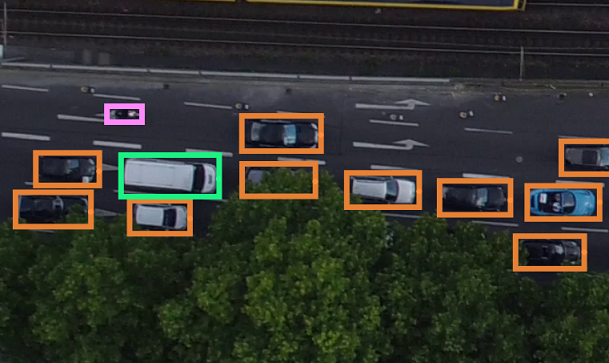
\includegraphics[width=0.45\linewidth]{resources/img/grundlagen/TrajectoryReconstruction/challenges/Verdeckung}
    \caption[Fahrbahn Verdeckung]{Verdeckung einer Fahrbahn durch Baumkronen}
    \label{fig:grund_lane_occlusion}
\end{figure}

Fahrbahnverdeckungen haben häufig zur Folge, dass die Bewegungsbahnen von Fahrzeugen in den
Trajektoriedatensätzen unterbrochen sind.
Durch den Einsatz von Verfahren, welche die Position eines Fahrzeugs schätzen, beispielsweise
Kalman- oder Partikel-Filter, können Unterbrechungen in Trajektorien zum Teil verhindert werden.

\subsubsection*{Niedrige Aufnahmewinkel}

Auch niedrige Aufnahmewinkel sind eine Herausforderung bei der Rekonstruktion von Fahrzeugtrajektorien.
Abbildung \ref{fig:grund_low_angle_detection} zeigt die Detektion eines LKW's in einer Luftbeobachtung,
welche aus einem niedrigen Aufnahmewinkel erstellt wurde. Problematisch ist hier, dass anhand der Bounding-Box,
welche die Position des LKW's im Bild definiert, sich nur schlecht dessen reale Position auf der Straße ermitteln lässt.
Die Bounding-Box ragt weit über die Fahrspur hinaus, auf welcher sich der LKW befindet und auch deren Mittelpunkt
liegt nicht in der Mitte der Fahrspur. Wenn Fahrzeugpositionen in Bildern mit niedrigem Aufnahmewinkel daher lediglich
anhand der Mittelpunkte der Bounding-Boxes ermittelt werden, weichen diese von den realen Positionen immer etwas ab.

\begin{figure}[H]
    \centering
    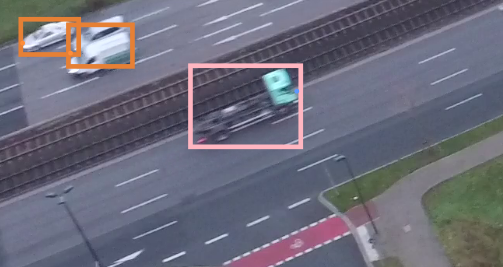
\includegraphics[width=0.45\linewidth]{resources/img/grundlagen/TrajectoryReconstruction/challenges/low_angle}
    \caption{Fahrzeug-Detektion bei niedrigem Aufnahmewinkel}
    \label{fig:grund_low_angle_detection}
\end{figure}

Beim Arbeiten mit Trajektoriedaten muss beachtet werden, dass die oben beschriebenen Effekte auftreten
können. Ein Spurerkennungsalgorithmus muss daher auch mit ihnen umgehen können.



\chapter{Clusteranalysen}
\label{sec:tra_clustering}

Die Clusteranalyse (kurz Clustering) ist ein wichtiges Werkzeug aus dem Bereich Data-Mining und Machine-Learning,
welches zur Auswertung von Daten unterschiedlichster Art eingesetzt wird.
Sie stellt kein konkretes Vorgehen oder einen Algorithmus dar, sondern beschreibt ein
allgemeines Problem, welches auf unterschiedlichste Weise gelöst werden kann. Eine Definition ist nachfolgend
gegeben:

\begin{theorem}[Clusteranalyse]
    Die Clusteranalyse ist ein Verfahren, um Datenobjekte aufgrund ihrer Eigenschaften und Beziehungen
    untereinander so zu gruppieren, dass sich die Objekte einer Gruppe möglichst stark ähneln und sich
    von den Objekten anderer Gruppen möglichst stark unterscheiden. Die auf diese Art entstehenden
    Objektgruppen werden \textit{Cluster} genannt.
\end{theorem}

Je höher die \textit{Homogenität} in einem Cluster
und die \textit{Differenz} zwischen den Clustern, desto besser ist die gewählte Clustering-Methode.
Der Einsatz einer Clusteranalyse ist in vielen Anwendungsgebieten und in unterschiedlichen wissenschaftlichen
Disziplinen sehr beliebt, um ein Verständnis von Daten zu erhalten und um Muster in solchen zu identifizieren \cite[]{tan2007introduction}.
Die Clusteranalyse kommt so beispielsweise in der Bild- \cite[]{Pappas1992} und Dokumentverarbeitung \cite[]{Hammouda2004},
der IT-Sicherheit \cite[]{Portnoy2001} oder auch in Sozialen Netzwerken \cite[]{Handcock2007} zum Einsatz.

Die Clusteranalyse hat viel mit dem Problem der Klassifizierung von Daten gemein, insofern sie Datenobjekten
Label zuordnet. Im Gegensatz zu \textit{überwachten} Klassifizierungsansätzen, wie dem heute populären überwachten
Lernen, leiten Clusteralgorithmen die Label allerdings alleine aus den vorhandenen Daten ab.
Es kommen keine Vergleichsobjekte mit bekannten, händisch vergebenen Labeln zum Einsatz.
Aus diesem Grund wird die Clusteranalyse auch als \textit{unüberwachte Klassifizierung} bezeichnet. \cite[]{tan2007introduction}

Das Konzept eines \textit{Clusters} ist nicht genau definiert. Es existieren daher viele unterschiedliche Konzepte
und Algorithmen zur deren Identifikation, welche sich jeweils für andere Anwendungsfälle eignen und verschiedene Eigenschaften
besitzen. Neben der Wahl eines passenden Clusteralgorithmus ist auch die Auswahl des verwendeten Distanzmaßes wichtig.

\begin{theorem}[Distanzmaß]
    Ein Distanz- oder Ähnlichkeitsmaß definiert zahlenmäßig wie ``ähnlich'' beziehungsweise ``unähnlich''
    sich zwei Objekte sind. Auf Basis der ermittelten Distanz beziehungsweise ``Ähnlichkeit'' werden
    Cluster gebildet.
\end{theorem}

Clustering ist kein selbsttätiger Prozess, welcher sich in
einheitlicher Weise auf unterschiedliche Probleme anwenden lässt. Jedes Problem erfordert die individuelle und sorgfältige
Auswahl eines passenden Algorithmus, eines Distanzmaßes und der richtigen Parameter. Die Bestimmung dieser geschieht
iterativ und nicht selten nach dem Prinzip des \textit{Trial and Error}. In Abbildung \ref{fig:grund_clustering_example}
ist beispielhaft ein Datensatz (links) mit -- für den Menschen intuitiv ersichtlich -- 7 unterschiedlichen Clustern (rechts)
dargestellt. Nach \cite[]{Jain2010} kann allerdings kein existierender Clustering Algorithmus diese alle erkennen.
\cite[]{Jain1999, tan2007introduction}

\begin{figure}[H]
    \centering
    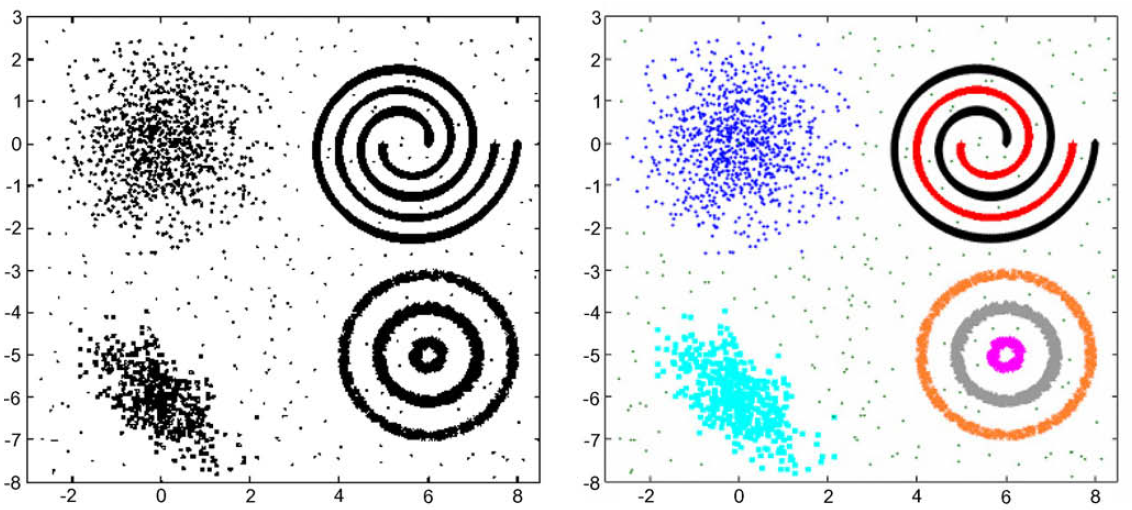
\includegraphics[width=0.8\linewidth]{resources/img/grundlagen/clustering_example}
    \caption[Rohdaten und erwünschtes Clustering-Ergebnis]{Rohdaten (links) und erwünschtes Clustering-Ergebnis (rechts) \cite[]{Jain2010}}
    \label{fig:grund_clustering_example}
\end{figure}

Aufgrund der Einschränkungen, welche alle Clusteralgorithmen besitzen, muss der Analyst sich vor deren Anwendung intensiv
mit den zu verarbeitenden Daten beschäftigen. Er muss ein Verständnis dafür besitzen, welche Struktur die Daten
haben, beziehungsweise annehmen können, und nach welchen Mustern zu suchen ist.
Besonders wichtiger ist zudem auch die Auswahl der richtigen, also relevanten, Datenmerkmale (\textit{``Feature Selection''})
und die Wahl deren Repräsentation (\textit{``Feature Transformation''}).
Nach der Selektion und Transformation der Daten müssen diese in einem Vorverarbeitungsschritt von eventuell auftretenden
und unerwünschten Effekten befreit werden. Dieser Schritt hat einen maßgeblichen Einfluss auf die Qualität
des finalen Clustering-Ergebnisses. Basierend auf vorangegangener Beschreibung und \cite[]{Jain1999},
lässt sich der grundlegende Ablauf einer Clusteranalyse wie folgt darstellen: \\

\begin{figure}[H]
    \centering
    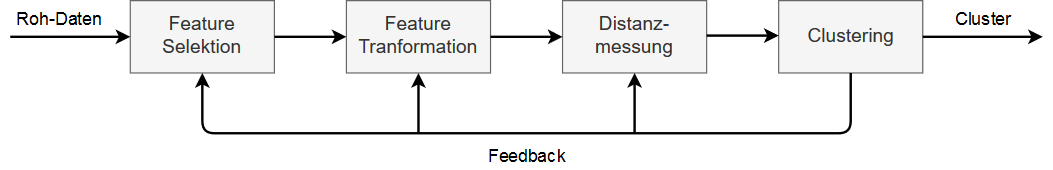
\includegraphics[width=\linewidth]{resources/img/grundlagen/clustering_flow}
    \caption[Ablauf einer Clusteranalyse]{Schrittweiser Ablauf einer Clusteranalyse}
    \label{fig:grund_clustering_workflow}
\end{figure}

\cite[]{Jain2010} nennt einige weitere Herausforderungen, welche bei der Durchführung einer Clusteranalyse berücksichtigt werden müssen:

\begin{enumerate}
    \item Daten können Ausreißer enthalten. Wie sollen diese behandelt werden?
    \item Die Anzahl der Zielcluster ist üblicherweise nicht bekannt. Wie kann sie im voraus bestimmt werden, wenn die Analyse es erfordert?
    \item Wie können gefundenen Cluster validiert werden?
\end{enumerate}

\section{Cluster-Sets und Cluster}

Cluster-Sets, das heißt die Gesamtheit aller durch eine Analyse gefundenen Cluster, und einzelnen Cluster selbst,
können in verschiedene Kategorien unterteilt werden beziehungsweise unterschiedliche Eigenschaften besitzen.
Nachfolgend sind die wichtigsten, basierend auf \cite[]{tan2007introduction}, \cite[]{Jain1999} und \cite[]{Jain2010}, aufgeführt.

\subsection{Eigenschaften von Cluster-Sets}
\label{sec:grund_property_cluster_sets}

Bei Cluster-Sets kann grundsätzlich zwischen folgenden Kategorien unterschieden werden.

\paragraph{Hierarchisch vs. Partitioniert}
Von \textit{hierarchischen} Cluster-Sets wird gesprochen, wenn die einzelnen Cluster verschachtelt sind und dadurch eine
Baum-Struktur bilden. Cluster sind hingegen \textit{partitioniert}, wenn keine Überlagerungen zwischen ihnen existieren.

\paragraph{Exklusiv vs. Überlappend vs. Fuzzy}
\textit{Exklusive} Cluster-Sets liegen vor, wenn jedem Datenwert ein oder kein Zielcluster zugeordnet wird.
Im Gegensatz hierzu können bei \textit{überlappenden} Cluster-Sets Objekte einer oder mehrerer Gruppen angehören.
Bei sogenannten \textit{Fuzzy} oder \textit{Soft} Cluster-Sets, gehört ein Datenobjekt einem Cluster
mit einer bestimmten Wahrscheinlichkeit oder Gewichtung an. Algorithmen, welche Daten eine
Wahrscheinlichkeit für die Zugehörigkeit zu einem Cluster zuweisen, werden \textit{probabilistische}
Clusteralgorithmen genannt.

\paragraph{Komplett vs. Partielle}
Von \textit{kompletten} Cluster-Sets wird gesprochen, wenn jedes Element der Eingangsdaten einem Cluster zugeordnet wird.
Bei \textit{partiellen} Sets ist dies nicht der Fall. Hier kann ein bestimmter Anteil an Datenwerten als Ausreißer markiert
werden, welche keine Gruppe besitzen.

\subsection{Eigenschaften von Clustern}

Da, wie oben erwähnt, das Konzept eines Clusters nicht klar definiert ist, können auch diese unterschiedliche
Eigenschaften besitzen. Die wichtigsten Cluster-Arten sind nachfolgend erläutert.

\paragraph{Klar separierte Cluster}
In einem \textit{klar separierten} Cluster besitzt jedes Datenobjekt einen geringeren Abstand zu allen anderen
Objekten der Gruppe, also zu Elementen außerhalb des Clusters.
Dargestellt ist dies in Abbildung \ref{fig:basic_cluster_style} a). Diese idealistische Definition eines
Clusters ist nur dann erfüllt, wenn die in den Daten enthaltenen Cluster einen großen Abstand voneinander haben.
In der Realität ist dies selten der Fall.

\paragraph{Prototyp-basierte Cluster}
Von einem \textit{Prototyp-basierten} Cluster wird gesprochen, wenn alle Elemente einer Gruppe einen
geringeren Abstand zu einem Prototyp oder Referenzwert des Clusters besitzen, als zu denen anderer
Gruppierungen (siehe Abb. \ref{fig:basic_cluster_style} b)).
Ein solcher Prototyp ist üblicherweise der Mittelwert der Datenelemente eines Clusters (\textit{Centroid}).

\paragraph{Graphen-basierte Cluster}
Die Definition eines \textit{Graphen-basierten} Clusters kann immer dann verwendet werden, wenn Daten
als vernetzter Graph dargestellt werden. In einem solchen sind die Elemente Knoten und die Kanten
repräsentieren Beziehungen zwischen ihnen. Ein Cluster in einem solchen Graphen ist definiert als Menge von
Knoten, welche untereinander verbunden sind, jedoch keine Verbindungen zu Elementen außerhalb des Clusters haben.
Dargestellt ist dies in Abbildung \ref{fig:basic_cluster_style} c).

\paragraph{Dichte-basierte Cluster}
\textit{Dichte-basierte} Cluster sind definiert als Regionen mit einer hohen Dichte an Objekten, welche von
Regionen umgeben sind, welche eine geringe Objektdichte besitzen (siehe Abb. \ref{fig:basic_cluster_style} d)).
Elemente, welche in einer solchen Region mit geringer Dichte liegen, werden als Ausreißer interpretiert.
Bereiche mit hoher Objektdichte werden üblicherweise gefunden, indem die Nachbarschaften von Elementen untersucht werden.

\paragraph{Konzeptionelle Cluster}
Eine sehr allgemeine Definition eines Clusters ist die der \textit{konzeptionellen} Gruppen. Hiermit ist
gemeint, dass die Elemente eines Clusters eine gemeinsame Eigenschaft besitzen. Dies schließt alle oben genannten
Cluster-Arten mit ein, lässt sich allerdings beliebig erweitern. So sind beispielsweise in Abbildung \ref{fig:basic_cluster_style} e)
konzeptionelle Cluster dargestellt, die die Form zweier Kreise und eines Rechtecks haben. Um solche Muster
erkennen zu können, benötigt ein Algorithmus ein spezielles ``Verständnis'' eines Clusters.

\begin{figure}[H]
    \centering
    \subfloat[Klar separierte Cluster]{{
        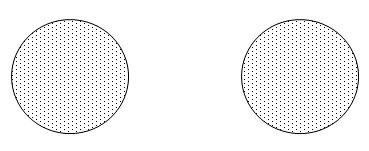
\includegraphics[align=c, width=0.3\linewidth]{resources/img/grundlagen/cluster/Cluster01}
    }}
    \qquad
    \qquad
    \subfloat[Centroid-basierte Cluster]{{
        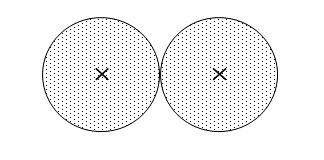
\includegraphics[align=c, width=0.3\linewidth]{resources/img/grundlagen/cluster/Cluster02}
    }}
    \hfill
    \subfloat[Graphen-basierte Cluster]{{
        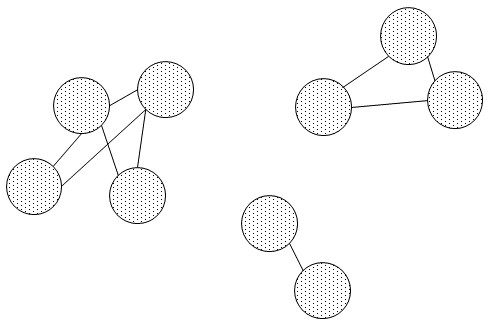
\includegraphics[align=c, width=0.3\linewidth]{resources/img/grundlagen/cluster/Cluster03}
    }}
    \qquad
    \qquad
    \subfloat[Dichte-basierte Cluster]{{
        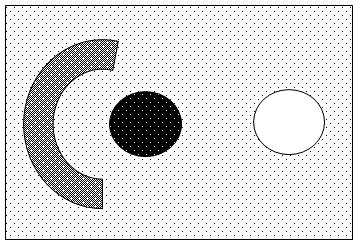
\includegraphics[align=c, width=0.3\linewidth]{resources/img/grundlagen/cluster/Cluster04}
    }}
    \hfill
    \subfloat[Konzeptionelle Cluster]{{
        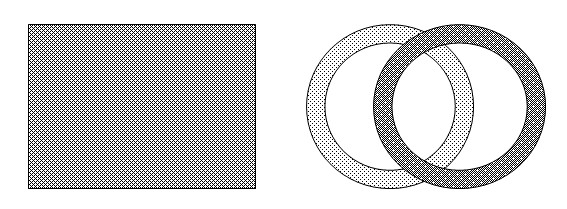
\includegraphics[align=c, width=0.6\linewidth]{resources/img/grundlagen/cluster/Cluster05}
    }}
    \caption[Visualisierung verschiedener Clusterarten]
            {Visualisierung verschiedener Clusterarten (basierend auf \cite[]{tan2007introduction})}
    \label{fig:basic_cluster_style}
\end{figure}

\section{Clusteralgorithmen}
\label{sec:cluster_algos}

Um mit den oben beschriebenen unterschiedlichen Cluster-Sets und Cluster Definitionen umgehen zu können,
existieren verschiedene Clustering-Modelle.
Einige wichtige Clustering-Ansätze sind Vernetzungsmodelle, Prototyp-Modelle, Verteilungsmodelle
und Dichtemodelle \cite[]{tan2007introduction, SauravKaushik2016}. Für jede Kategorie existieren unterschiedliche Algorithmen. Im Folgenden werden
diese Modelle und jeweils exemplarisch ein Algorithmus vorgestellt.

\subsection{Vernetzungsmodelle}
\label{sec:grund_vernetzungs_clustering}

Vernetzungsmodelle werden auch häufig \textit{hierarchische Cluster-Modelle} genannt. Sie beruhen auf
der Annahme, dass Elemente, welche nahe beieinander liegen, eine höhere Gemeinsamkeit besitzen als solche,
welche weiter voneinander entfernt sind. Zur Bestimmung der Nähe zwischen Elementen benötigen Vernetzungsmodelle,
wie auch andere Cluster-Modelle, eine Verständnis von Distanz. Dieses wird über ein \textit{Distanzmaß} definiert.
Zusätzlich ist ein \textit{Link-Kriterium} notwendig,
welches bestimmt, wie genau die Entfernung zwischen zwei Clustern ermittelt wird. Übliche Link-Kriterien
sind \textit{Minimum-Linkage}, welches die minimale Distanz zwischen den Objekten der Cluster als Distanz verwendet,
oder \textit{Maximum-Linkage} beziehungsweise \textit{Average-Linkage}. \cite[]{Jain1999, GeorgeSeif2018}

Grundsätzlich teilen sich hierarchische Clusteralgorithmen in zwei Gruppen auf:
\textit{Agglomerative} (Bottom-Up) und \textit{Divisive} (Top-Down) Algorithmen.
Agglomerative Ansätze weisen zu Beginn des Clustervorgangs jedem Datenelement eine eigene Gruppe zu
und vereinen diese anschließend.
Bei divisiven Ansätzen werden hingegen zu Beginn alle Elemente in einem Cluster zusammengefasst und
diese in den nachfolgenden Schritten geteilt. \cite[]{SauravKaushik2016}

Als Beispiel wird anschließend der \textit{agglomerative-hierarchische Clusteralgorithmus} genauer vorgestellt.
Seine Arbeitsweise lässt sich sehr gut anhand sogenannter Dendrogramme oder geschachtelter Cluster-Diagramme darstellen
(siehe Abbildung \ref{fig:grund_agglo_clustering}).

\begin{figure}[H]
    \centering
    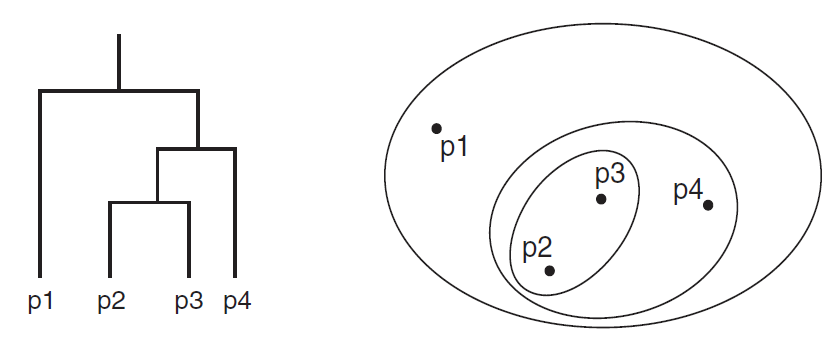
\includegraphics[width=0.7\linewidth]{resources/img/grundlagen/agglo_clustering}
    \caption[Darstellung Funktionsweise Agglomeratives Clustering]
            {Agglomeratives Clustering dargestellt als Dendrogramm (links) und geschachteltes Cluster-Diagram (rechts) \cite[]{tan2007introduction}}
    \label{fig:grund_agglo_clustering}
\end{figure}

Im ersten Schritt des Algorithmus werden alle Datenpunkte als separate Cluster markiert. Diesen Schritt
repräsentieren die Blätter des Dendrogramms.
Anschließend muss ein Distanzmaß und ein Link-Kriterium gewählt werden.
Das am häufigsten verwendete Distanzmaß ist sicherlich der euklidsche Abstand, welcher die Distanz zwischen zwei Punkten
oder Vektoren im $n$-dimensionalen Raum bestimmt. Er ist definiert durch Formel \ref{eq_dist}.

\begin{ceqn}
\begin{align}
\label{eq_dist}
    dist(p,q) = ||q-p||_2 = \sqrt{\sum_{i=1}^n (q_i-p_i)^2}
\end{align}
\end{ceqn}

Wird als Link-Kriterium beispielsweise \textit{Minimum-Linkage} gewählt, ist dieses definiert als:

\begin{ceqn}
\begin{align}
\label{eq_linkage}
    link(P, Q) = min\{ dist(p,q)\ |\ p \in P, q \in Q\}
\end{align}
\end{ceqn}

Hierbei entsprechen $P$ und $Q$ zwei Clustern, welche die Elemente $p \in P$ und $q \in Q$ enthalten.
Auf Basis des gewählten Link-Kriteriums kann nun eine Distanz-Matrix für die einzelnen Cluster
erstellt werden.
Die zwei Cluster mit minimalem Abstand voneinander werden anschließend zusammengeführt und die
vorherigen Schritte werden wiederholt, bis nur noch ein Cluster (Wurzel des Dendrogramms) beziehungsweise
die gewünschte Clusteranzahl übrig ist. \cite[]{GeorgeSeif2018, tan2007introduction}

Bei den meisten Varianten des agglomerativen Clusterings muss der Nutzer die Anzahl der Zielcluster im
vorraus festlegen, was problematisch ist, da diese meist nicht bekannt ist. Umgangen werden kann dies nur,
indem ein Link-Kriterium gewählt wird, das ab einer bestimmten Distanz zwischen den Clustern diese nicht weiter
fusioniert \cite[]{GeorgeSeif2018}.

Die Zeitkomplexität des agglomerativen Clusterings beträgt bestenfalls $O(n^2log\ n)$ weshalb die Menge der Daten,
welche mit ihm verarbeitet werden können, erheblich begrenzt ist \cite[]{tan2007introduction}.

\subsection{Prototyp-Modelle}
\label{sec:grund_prototype_clustering}

Prototyp-basierte Clustering-Modelle betrachten im Gegensatz zu hierarchischen Modellen nicht die Distanz
zwischen Clustern, sondern die Entfernung von Objekten zu Referenzpunkten, den \textit{Prototypen}.
Die am häufigsten verwendeten Prototypen sind \textit{Centroids}, welche den Mittelpunkt eines Clusters dargestellen.
\textit{Medoids}, welche teilweise auch genutz werden, repräsentieren hingegen den Median eines Clusters. \cite[]{tan2007introduction}

Ein Beispiel für einen Centroid-Clusteralgorithmus ist \textit{k-Means}. Dieser ist aufgrund seines Alters,
seiner Einfachheit und der vielen Weiterentwicklungen wohl der bekannteste Clusteralgorithmus überhaupt.

Das Ziel von k-Means ist es, für eine n-dimensionale Punktmenge $X = \{ x_1 ... x_n \}$ ein Cluster-Set $C = \{ c_1 ... c_k \}$
zu finden, welches die Summe der quadratischen Abweichung (Gleichung \ref{eq_kmeans1}) zwischen allein Punkten in einem Cluster und deren
Mittelwerte $\mu_k$ (Centroids) minimiert.

\begin{ceqn}
\begin{align}
    \label{eq_kmeans1}
    J(c_k) = \sum_{k=1}^K \sum_{x_i \in c_k} || x_i - \mu_k ||^2
\end{align}
\end{ceqn}

Eine Lösung für dieses Problem zu finden, ist NP-Schwer. Aus diesem Grund
ist k-Means ein approximativer Ansatz, welcher nicht garantieren kann, ein globales Minimum zu finden \cite[]{Jain2010}.
Die Funktionsweise des Algorithmus ist in Abbildung \ref{fig:grund_kmeans_clustering} dargestellt.
Die Kreuze entsprechen hierbei den Centroids, welche sich in jeder Iterationen in Richtung der
Clustermittelpunkte verschieben.

\begin{figure}[H]
    \centering
    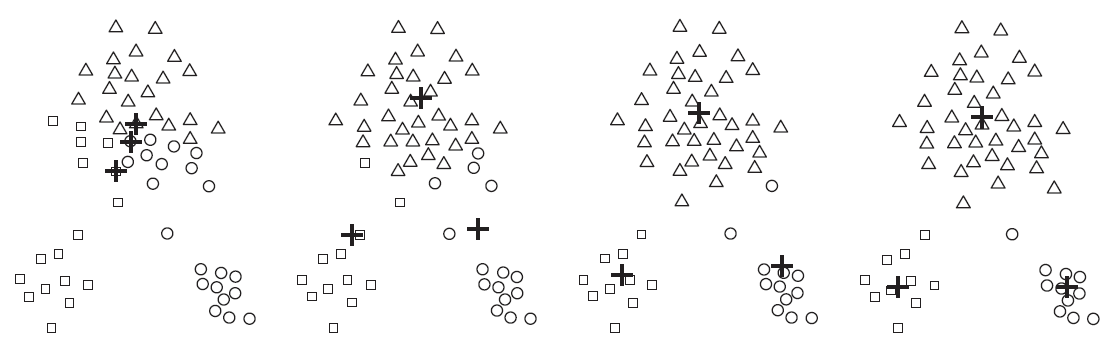
\includegraphics[width=0.9\linewidth]{resources/img/grundlagen/k-means}
    \caption[Funktionsweise k-Means Clusteralgorithmus]
            {Funktionsweise k-Means Clusteralgorithmus über mehrere Iterationen \cite[]{tan2007introduction}}
    \label{fig:grund_kmeans_clustering}
\end{figure}

Ausgehend von der Punktmenge $X$ und der gesuchten Cluster-Anzahl $k$,
werden im ersten Schritt $k$ zufällig positionierte Centroids $\mu_k$ definiert.
Anschließend wird für alle Punkte $x_i$ der nächstgelegene Centroid $\mu_j$ gesucht.

\begin{ceqn}
\begin{align}
    \label{eq_kmeans2}
    j = arg\ min(dist(x_i, \mu_j))
\end{align}
\end{ceqn}

$x_i$ wird daraufhin Mitglied in Cluster $C_j$. Als Distanzmaß ($dist$) kann hier wieder der euklidsche Abstand
(Gleichung \ref{eq_dist}) verwendet werden oder aber auch beliebige andere Maße.
Nachdem alle Punkte $x_i$ einem Cluster zugewiesen wurden, werden die Centroid Positionen neu bestimmt.
Hierzu wird der Durchschnitt aller Punkte eines Clusters berechnet:

\begin{ceqn}
\begin{align}
    \label{eq_kmeans3}
    c_j = \frac{1}{n} \sum_{x_j \in C_j} x_j
\end{align}
\end{ceqn}

Diese zwei Schritte werden mehrfach wiederholt, bis das Ergebnis konvergiert, das heißt die Zuweisungen sich
nurnoch geringfügig ändern. \cite[]{Jain2010}

Der größte Nachteil des k-Means Algorithmus ist, das auch bei ihm die Anzahl der Zielcluster spezifiziert
werden muss. Des Weiteren ist sein Ergebnis aufgrund der zufälligen Initialisierung der Centroids
nicht deterministisch. Ein Vorteil von k-Means ist hingegen, dass seine Zeitkomplexität bei $O(n)$ liegt. \cite[]{tan2007introduction}

Um die genannten Nachteile, zumindest in Teilen, umgehen zu können, existieren diverse Weiterentwicklungen des k-Mean
Algorithmus. So stammen beispielsweise von \cite[]{Hamerly} und \cite[]{Pelleg} die Algorithmen \textit{g-Means}
beziehungsweise \textit{x-Means}, welche die Clusteranzahl $k$ auf Basis mehrerer k-Means Durchläufe und
statistischer Kennzahlen bestimmen.

\subsection{Verteilungsmodelle}
\label{sec:grund_distribution_clustering}

Verteilungs-Clustering-Modelle basieren auf der Verwendung von statistischen Wahrscheinlichkeitsverteilungen wie
beispielsweise der Gauß-Verteilung. Cluster werden darüber definiert, wie wahrscheinlich es ist, dass Objekte
der selben Verteilung angehören. Problematisch ist die Verwendung dieser Clustering-Methodik, da sie anfällig für
das Problem des \textit{``Overfitting''} ist, wenn die Komplexität der verwendeten Modelle nicht beschränkt wird.
Zudem ist die Annahme, dass vielen realen Datensätzen ein statistisches Verteilungsmodell zugrundeliegt, gefährlich.
Ist diese These jedoch berechtigt, dann haben die Modelle den Vorteil, dass sie neben der Zuweisung von Objekten zu Clustern
auch Korrelationen zwischen einzelnen Attributen aufzeigen können. \cite[]{AndersDrachen2014}

Nachfolgend wird der bekannteste Vertreter der Verteilungs-Clusteralgorithmen vorgestellt:
das \textit{Expectation–maximization} (\acrshort*{em}) Verfahren unter Verwendung sogenannter \textit{Gaus-sian-Mixture-Models} (\acrshort*{gmm}).
Die Funktionsweise des EM-Algorithmus hat grundsätzlich viel gemein mit der des k-Mean Algorithmus.
Es wird ebenfalls mit einer festen Anzahl zufällig initialisierter Modelle gestartet, welche anschließend über mehrere Iterationen
hinweg an die Daten angepasst werden. Im Gegensatz zu k-Means, sind die gewählten Modelle hingegen Gauß-Verteilungen,
welche zwei Parameter besitzen: ihren Mittelwert und die Standardabweichung.
Das Vorgehen des EM-Algorithmus ist nachfolgend, basierend auf \cite[]{GeorgeSeif2018}, beschrieben und in
Abbildung \ref{fig:grund_em_clustering} grafisch dargestellt.

\begin{enumerate}
    \item Wahl der Clusteranzahl $k$ und Initialisierung der Gauß-Modelle für die entsprechenden Cluster.
    \item Berechnung der Wahrscheinlichkeit, dass ein Datenpunkt zu einem Cluster gehört. Je näher
              ein Datenpunkt dem Zentrum einer Gauß-Verteilung ist, desto höher die Wahrscheinlichkeit für dessen Zugehörigkeit.
    \item Basierend auf den Wahrscheinlichkeiten werden die Parameter der Verteilungen neu berechnet.
              Hierzu wird die gewichtete Summe der Datenpunkt-Positionen errechnet. Die Gewichte entsprechen dabei
              den Wahrscheinlichkeiten, dass ein Element zu einem Cluster gehört. Hierdurch werden die Gauß-Modelle automatisch
              den in den Daten enthaltenen Clustern angepasst.
    \item Wiederholdung der Schritte 2) und 3), bis das Clustering-Ergebnis konvergiert.
\end{enumerate}

\begin{figure}[H]
    \centering
    \subfloat[Iteration 1]{{
        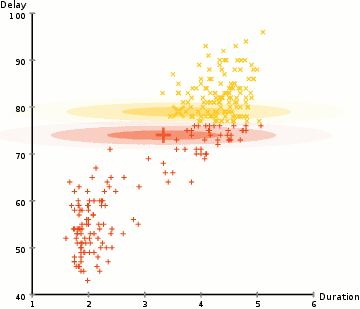
\includegraphics[align=c, width=0.22\linewidth]{resources/img/grundlagen/clustering_EM/EM1}
    }}
    \subfloat[Iteration 2]{{
        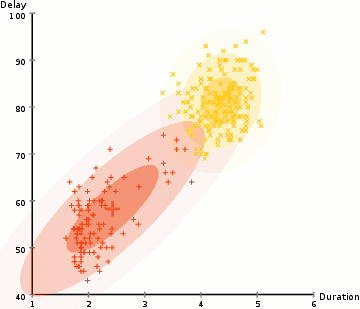
\includegraphics[align=c, width=0.22\linewidth]{resources/img/grundlagen/clustering_EM/EM2}
    }}
    \subfloat[Iteration 3]{{
        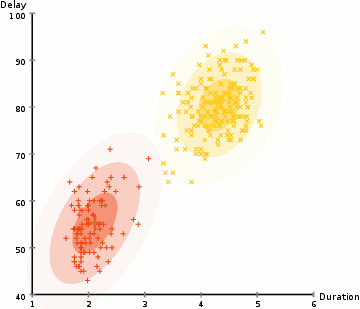
\includegraphics[align=c, width=0.22\linewidth]{resources/img/grundlagen/clustering_EM/EM3}
    }}
    \subfloat[Iteration 4]{{
        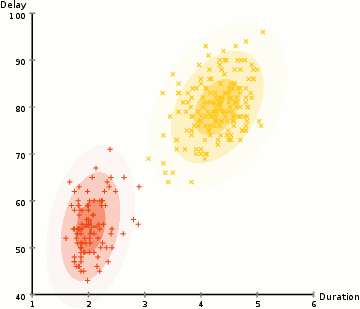
\includegraphics[align=c, width=0.22\linewidth]{resources/img/grundlagen/clustering_EM/EM4}
    }}
    \caption[Funktionsweise des EM-Clusteralgorithmus]{Funktionsweise des EM-Clusteralgorithmus über mehrere Iterationen \cite[]{GeorgeSeif2018}}
    \label{fig:grund_em_clustering}
\end{figure}

Ziel des EM-Algorithmus ist es, die Parameter der Gauß-Modelle so zu optimieren, dass diese die Verteilung
der Daten bestmöglich beschreiben. Am Ende des Clusterings besitzt jeder Datenwert die Zugehörigkeits-Wahrscheinlichkeiten
für die einzelnen Cluster. Ein Element wird jenem Cluster zugeordnet, für welches es die höchste
Wahrscheinlichkeit besitzt.

\subsection{Dichtemodelle}
\label{sec:grund_density_clustering}

Dichte-basierte Cluster sind, wie oben beschrieben, definiert als Regionen hoher Objektdichte, welche
von Bereichen geringer Dichte umgeben sind. Dichte-Clustering-Modelle suchen nach eben solchen Regionen.
Großer Vorteil der Algorithmen dieser Klasse ist, dass sie Cluster beliebiger Formen identifizieren können,
nicht auf die Vorgabe einer Clusteranzahl angewiesen sind und mit Ausreißern umgehen können. \cite[]{tan2007introduction}

Als Vertreter der Dichte-basierten Ansätze wird nachfolgend der \textit{\acrshort*{dbscan}} Algorithmus
(\textit{Density-Based Spatial Clustering of Applications with Noise}), wie in \cite[]{Gao2012} beschrieben, vorgestellt.
Er verwendet als Maß für die Dichte einer Region die sogenannte \textit{$\epsilon$ -Nachbarschaft} $N_{\epsilon}$.
Diese selektiert für ein Objekt $p$ alle Objekte, welche innerhalb des Radius $\epsilon$ um dieses liegen:

\begin{ceqn}
\begin{align}
    \label{eq_dbscan_1}
    N_{\epsilon}(p) = \{ q\ |\ dist(p,q) \leq \epsilon \}
\end{align}
\end{ceqn}

Eine $\epsilon$-Nachbarschaft besitzt eine hohe Dichte, wenn in ihr mindestens $MinPts$ Objekte liegen.

Basierend auf der Definition von $N_{\epsilon}$, werden die in einem Datensatz vorhandenen Elemente in
drei Klassen unterteilt. Sie sind entweder \textit{Kern-}, \textit{Rand-} oder \textit{Ausreißer-} Objekte.
Ein Kernobjekt hat mindestens $MinPts$ andere Punkte in $N_{\epsilon}$.
Randobjekte besitzen weniger als $MinPts$ in $N_{\epsilon}$, liegen aber in der Nachbarschaft eines Kernobjektes.
Ausreißerobjekte sind weder Kern- noch Randobjekte.

\begin{figure}[H]
    \centering
    \subfloat[]{{
        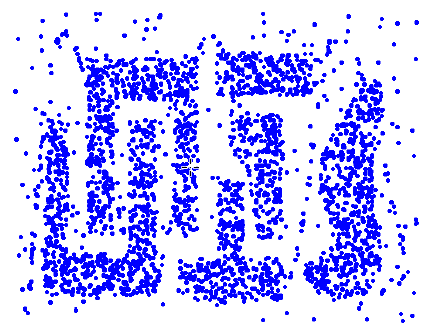
\includegraphics[align=c, width=0.3\linewidth]{resources/img/grundlagen/clustering_dbscan/dbscan1}
    }}
    \subfloat[]{{
        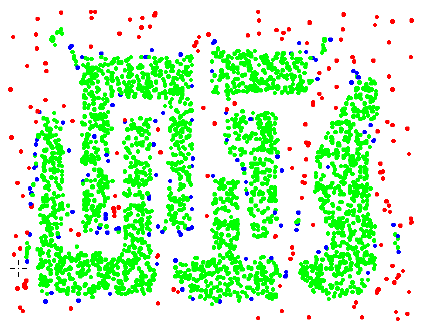
\includegraphics[align=c, width=0.3\linewidth]{resources/img/grundlagen/clustering_dbscan/dbscan2}
    }}
    \subfloat[]{{
        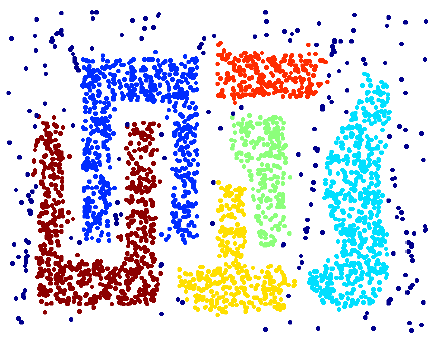
\includegraphics[align=c, width=0.3\linewidth]{resources/img/grundlagen/clustering_dbscan/dbscan3}
    }}
    \caption[Schritte des DBSCAN Algorithmus]
            {Schritte des DBSCAN Algorithmus, a) Rohdaten, b) Klassifizierung in Kern- (grün), Rand- (blau) und Ausreißer- (rot) Punkte, c) Clustering Ergebnis \cite[]{Gao2012}}
    \label{fig:grund_dbscan_clustering}
\end{figure}

Auf Basis der drei Objektklassen lässt sich das Prinzip der Dichte-basierten \textit{Erreichbarkeit} definieren.
Ein Objekt $q$ ist von $p$ \textit{direkt} erreichbar, wenn $p$ ein Kernobjekt ist und $q$ in dessen $N_{\epsilon}$ liegt.
In Abbildung \ref{fig:grund_dbscan_reachability} gilt dies beispielsweise für $p$ und $p_2$.
Zwei Elemente sind \textit{indirekt} erreichbar, wenn sie über eine Reihe von Zwischenschritten indirekt
verbunden sind (transitiv). Dies ist in Abbildung \ref{fig:grund_dbscan_reachability} für $q$ und $p$ der Fall.

\begin{figure}[H]
    \centering
    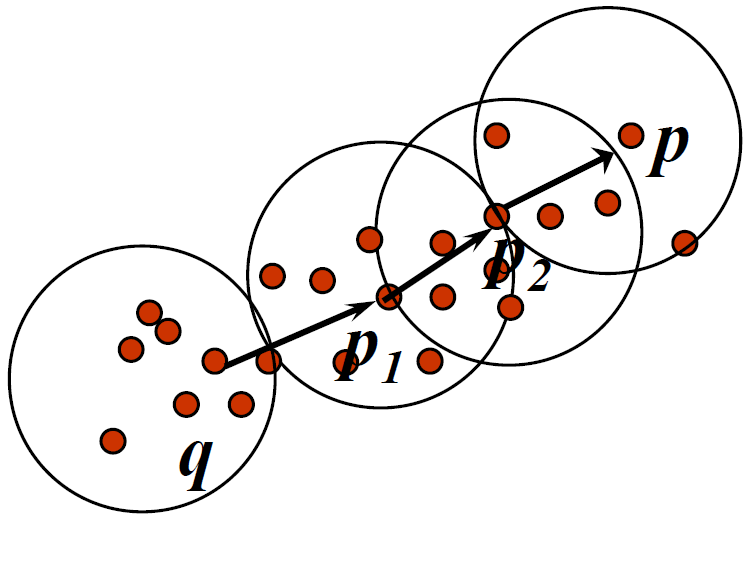
\includegraphics[width=0.32\linewidth]{resources/img/grundlagen/clustering_dbscan/reachability}
    \caption[Konzept Erreichbarkeit in DBSCAN]
            {Konzept der Dichte-basierten Erreichbarkeit in DBSCAN \cite[]{Gao2012}}
    \label{fig:grund_dbscan_reachability}
\end{figure}

Der DBSCAN Algorithmus kann, basierend auf den obigen Definitionen, wie folgt beschrieben werden:

\begin{enumerate}
    \item Unterteilung der Objekte in die drei Objektklassen (vgl. Abb. \ref{fig:grund_dbscan_clustering} b)).
    \item Aussortierung der Ausreißer-Objekte.
    \item Wahl eines nicht zugewiesenen Kernobjektes.
    \item Erstellung eines neuen Clusters für das Kernobjekt und alle von ihm ausgehend direkt und indirekt erreichbaren Objekte.
    \item Wiederholdung der Schritte 3) und 4), bis alle Kern- und Randobjekte einem Cluster zugewiesen sind. (vgl. Abb. \ref{fig:grund_dbscan_clustering} c))
\end{enumerate}

DBSCAN besitzt die oben erwähnten Vorteile Dichte-basierter Clusteralgorithmen. Dank einer Zeitkomplexität
von $O(n\ log\ n)$, kann er außerdem auch auf große Datensätze angewendet werden \cite[]{tan2007introduction}.
Nachteil des Ansatzes ist, dass er schlecht mit Clustern umgehen kann, welche unterschiedliche Dichten besitzen.

\section{Distanzmaße zum Vergleich von Fahrzeugtrajektorien}
\label{sec:distance_measures}

Bei der Clusteranalyse ist neben der Wahl des passenden Clusteralgorithmus insbesondere
die Entscheidung, welches Distanzmaß verwendet wird, ausschlaggebend.
Im obigen Abschnitt wurde bereits die euklidsche Distanz (Gleichung \ref{eq_dist}) als ein mögliches Distanzmaß
vorgestellt. Dieses kann jedoch nur zur Bestimmung der Distanz zwischen $n$-dimensionalen Punkten im euklidschen Raum verwendet
werden. Dasselbe gilt für andere einfache Maße wie die Manhatten-Distanz oder die Pearson-Distanz.

Um Fahrzeugtrajektorien korrekt gruppieren zu können, ist ein Distanzmaß notwendig, welches, je nach Anforderungen,
die unterschiedlichen Aspekte der Trajektorien vergleicht. Häufig werden die Eigenschaften Lage, Form und Länge
hierzu herangezogen. In der Literatur werden diverse Maße zum Vergleich von Trajektorien vorgestellt. Diese besitzen
alle unterschiedliche Eigenschaften, Vor- und Nachteile.

Nachfolgend werden exemplarisch drei Distanzmaße vorgestellt, anhand welcher ersichtlich ist, welche Abwägungen
bei der Wahl des Maßes gemacht werden müssen.
In allen drei Fällen werden die Trajektorien als Reihen zwei-dimensionaler Punkte mit Länge $n$ interpretiert:
$t_i = \{(x_1, y_1), (x_2, y_2), ..., (x_n, y_n)\}$.
Der $n$-te Punkt einer Trajektorie ist gegeben über $t_i(n)$ und deren Punkt-Länge über $len(t_i)$.
Die Menge der zu vergleichenden Trajektorien ist $T = \{t_1, t_2, ..., t_m\}$.
Abbildung \ref{fig:grund_trajectories} zeigt beispielhaft eine Auswahl von Trajektorien mit
unterschiedlichen Bewegungsmustern.

\begin{figure}[H]
    \centering
    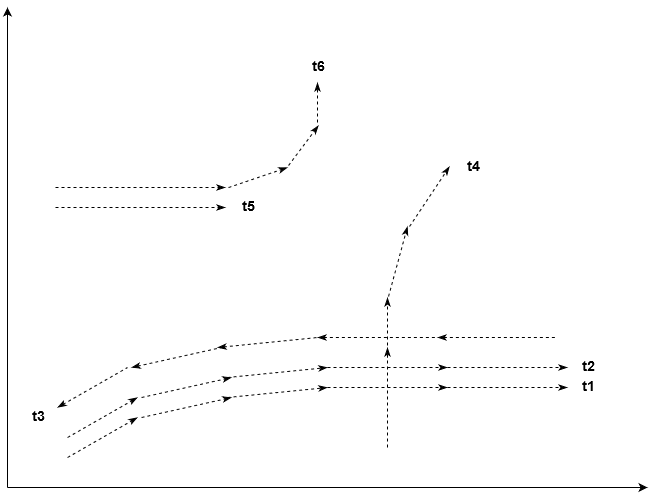
\includegraphics[width=0.6\linewidth]{resources/img/grundlagen/trajectories}
    \caption{Trajektorien im zwei-dimensionalen Raum}
    \label{fig:grund_trajectories}
\end{figure}

\subsection{HU-Distanz}
\label{sec:hu_distance}

Die HU-Distanz wurde erstmals in der Arbeit \textit{``Similarity based vehicle trajectory clustering and anomaly detection''}
von \cite[]{Hu2005} vorgestellt. Es ist ein sehr einfaches Distanzmaß, welches auf der mittleren euklidschen Distanz
zwischen zwei Trajektorien basiert. Berechnet wird die HU-Distanz für zwei Trajektorien $t_1$ und $t_2$ wie folgt:

\begin{ceqn}
\begin{align}
\label{eq_hu_distance1}
    D_{HU}(t_1, t_2) &= \frac{1}{N} \sum_{n = 1}^N dist(t_1(n), t_2(n)) \\
\label{eq_hu_distance2}
    wobei\ N &= min(len(t_1), len(t_2))
\end{align}
\end{ceqn}

Aus dieser Formel lassen sich sowohl die Vor- als auch Nachteile der HU-Distanz ableiten. Der klare Vorteile der
HU-Distanz ist deren Einfachheit und die Effizienz von $O(n)$.
Nachteil ist hingegen, dass das Distanzmaß nur gut funktioniert, wenn die Trajektorien bestimmte
Kriterien erfüllen. So sollten Trajektorien, welche einem Cluster angehören, auch immer möglichst auf der selben Höhe beginnen,
damit deren mittlerer Abstand nicht, aufgrund einer Verschiebung, erhöht wird.
Außerdem ist es notwendig, die Abstände zwischen den Punkten der Trajektorien auf die selbe Länge zu bringen,
damit beim paarweisen Vergleich immer Elemente verglichen werden, welche gleichweit vom Start der
Trajektorien entfernt sind.

Diese Eigenschaften der Bewegungsbahnen müssen über einen Vorverarbeitungsschritt geschaffen werden.
Problematisch bei der Verwendung der HU-Distanz ist außerdem, dass beim Vergleich zweier Trajektorien immer nur
die ersten $N$ Punkte (s. Gleichung \ref{eq_hu_distance2}) betrachtet werden. Dies kann dazu führen, dass zwei
Trajektorien, welche anfangs fast identisch verlaufen und sich später voneinander entfernen, trotzdem einen hohen
Ähnlichkeitswert besitzen (vergleiche $t_5$ und $t_6$ in Abbildung \ref{fig:grund_trajectories}).

Die HU-Distanz kann aufgrund der genannten Einschränken nur in speziellen Fällen oder nach starker Vorverarbeitung
der Trajektorien angewandt werden. Sie liefert ansonsten schlechte Clustering Ergebnisse.

\subsection{Hausdorff-Distanz}
\label{sec:hausdorff_distance}

Die Hausdorff-Distanz ist ein komplexeres Maß zur Bestimmung der Ähnlichkeit zwischen zwei Trajektorien.
Sie misst grundsätzlich den Abstand zwischen zwei nicht-leeren, ungeordneten Teilmengen $A$ und $B$ und ist für
Trajektorien definiert über die Gleichungen \cite[]{Atev2010}:

\begin{ceqn}
\begin{align}
\label{eq_hausdorff1}
    D_{HD}(t_1, t_2) &= max(h(t_1, t_2), h(t_2, t_1)) \\
\label{eq_hausdorff2}
    h(t_1, t_2) &= \underset{i\ \in\ t_1}{max}\ \underset{j\ \in\ t_2}{min}\ dist(i, j)
\end{align}
\end{ceqn}

$h(t_1, t_2)$ wird als gerichtete Hausdorff-Distanz \textit{von} $t_1$ \textit{nach} $t_2$ bezeichnet.
Sie findet die maximale Distanz einer Trajektorie zum nächsten Punkt einer anderen Trajektorie \cite[]{Huttenlocher}.
Da $h$ gerichtet ist, gilt $h(t_1, t_2) \neq h(t_2, t_1)$. Aus diesem Grund wird die Hausdorff-Distanz
\textit{zwischen} zwei Trajektorien mittels $D_{HD}$ bestimmt. $dist$ kann ein beliebiges Maß für die Distanz zweier
Punkte sein, wie beispielsweise die euklidsche Distanz.
Grundsätzlich lässt sich über die Hausdorff-Distanz die Form zweier Trajektorien vergleichen. Diese sind ähnlich,
wenn jeder Punkt einer Trajektorie einen nahegelegenen Punkt in der Vergleichsbahn besitzt.

Vorteil der Hausdorff-Distanz im Vergleich zur HU-Distanz ist, dass diese immer vollständige Trajektorien vergleicht
und nicht nur Teile. Außerdem ist bei ihrer Verwendung keine Vorverarbeitung in Form von Resampling et cetera notwendig.
Problematisch ist das Distanzmaß hingegen, da es mit ungeordneten Sets arbeitet und somit im Fall von Trajektorien deren
Orientierung nicht beachtet. Zwei parallele aber in entgegengesetzte Richtungen laufende Trajektorien, wie beispielsweise
die Trajektorien $t2$ und $t3$ in Abbildung \ref{fig:grund_trajectories}, würden nach Hausdorff eine hohe Ähnlichkeit besitzen.
Zudem kann das Distanzmaß schlecht mit Ausreißern umgehen, da bereits ein einzelner Ausreißer, bei ansonsten identischen
Trajektorien, zu einer beliebig kleinen Ähnlichkeit führen kann.
Von Nachteil ist auch, dass die Zeitkomplexität der Hausdorff-Distanz bei $O(n\ m)$ liegt.

\subsection{Longest-Common-Subsequence}
\label{sec:lcss_distance}

Das \textit{Longest-Common-Subsequence} (\acrshort*{lcss}) Distanzmaß basiert auf dem allgemeinen Problem der Findung
einer längsten gemeinsamen Subsequenz zwischen zwei Sequenzen. Da Trajektorien, nach obiger Definition, lediglich Punktsequenzen sind,
lässt sich das Verfahren sehr gut auf sie anwenden. Aufgrund von Erweiterungen des Basis-Algorithmus, besitzt
das LCSS Distanzmaß einige besondere Eigenschaften. Der Algorithmus für Trajektorien ist grundsätzlich
wie folgt definiert \cite[]{Vlachos2002}:

\begin{ceqn}
\begin{align}
\label{eq_lcss}
    LCSS_{\epsilon, \delta}(t_1, t_2) =
    \begin{cases}
        0 & \text{if } t_1 \text{ or } t_2 \in \emptyset \\
        1 + LCSS_{\epsilon, \delta}(t_1', t_2') & \text{if } dist(t_1(n), t_2(m)) < \epsilon \\
        & \land\ |n - m| \leq \delta \\
        max(LCSS_{\epsilon, \delta}(t_1', t_2), LCSS_{\epsilon, \delta}(t_1, t_2')) & \text{otherwise}
    \end{cases}
\end{align}
\end{ceqn}

Hierbei gilt $t_i' = \{ t_i(0),\ ...,\ t_i(n-1)\}$.
Die Parameter $\epsilon$ und $\delta$ bestimmen das
Vergleichsverhalten des Algorithmus. Über $\epsilon$ wird definiert, wieweit zwei Punkte maximal voneinander entfernt liegen
können, um immer noch als ``übereinstimmend'' zu gelten. $\delta$ bestimmt hingegen, wieweit in beide zeitliche Richtungen
gesucht wird, um einen übereinstimmenden Punkt zu finden.
Da die obige LCSS Funktion nur ein diskretes Zählmaß definiert, ist das eigentliche LCSS-Distanz üblicherweise
gegeben als \cite[]{Vlachos2002}:

\begin{ceqn}
\begin{align}
\label{eq_lcss_distance}
    D_{LCSS}(\delta, \epsilon, t_1, t_2) = 1 - \frac{LCSS_{\delta, \epsilon}(t_1, t_2)}{min(len(t_1), len(t_2))}
\end{align}
\end{ceqn}


Vorteil der LCSS Ähnlichkeitdefinition ist, dass sie mit kompletten Trajektorien arbeitet und robust
gegenüber Ausreißern ist, da nicht für alle Punkte Übereinstimmungen in den Trajektorien gefunden werden müssen.
Über $\epsilon$ und $\delta$ kann die ``Strenge'' des Algorithmus geregelt werden.
Zudem berücksichtigt das LCSS Maß die Orientierung der Trajektorien.
Die rekursive Definition des LCSS Algorithmus aus Gleichung \ref{eq_lcss} lässt sich mittels dynamischer Programmierung
und \textit{Memoisation} mit Zeitkomplexität $O(n\ m)$ berechnen.

\subsection{Wahl eines Distanzmaßes}

Anhand der drei ausgewählten und oben exemplarisch beschriebenen Distanzmaße ist bereits ersichtlich,
dass die Wahl eines passenden Maßes nicht trivial ist. Es muss die Qualität und Form der Daten berücksichtigt werden.
Außerdem muss abgewogen werden, in wieweit es möglich beziehungsweise gewünscht ist, die Daten vorzuverarbeiten.

Das primäre Auswahlkriterium ist natürlich die situationsabhängige Definition von ``Distanz'':
Sind sich Trajektorien ähnlich, wenn sie lediglich die selbe Form haben und ansonsten an beliebigen Stellen im Raum liegen?
Sind sie sich ähnlich, wenn sie die selbe Form haben und im Raum nahe beieinander liegen? Ist ihre Orientierung relevant?
Dies sind wichtige Fragen, welche vor der Wahl eines Distanzmaßes geklärt werden müssen.
Da die Maße als Distanzfunktionen bei der Clusteranalyse verwendet werden, ist ihr Verhalten ausschlaggebend
für den Erfolg der Gruppierung von Trajektorien.